\documentclass[11pt,a4paper]{article}

\usepackage[utf8]{inputenc}
\usepackage[T1]{fontenc}
\usepackage[english]{babel}
\usepackage[margin=1.5cm, top=1.5cm, bottom=1.5cm]{geometry}
\usepackage{graphicx}
\graphicspath{{../01_Propuesta/Logos/}{./}}
\usepackage{fancyhdr}
\usepackage{xcolor}
\usepackage[hidelinks]{hyperref}

\definecolor{verdeosc}{RGB}{26,107,60}
\definecolor{verdemid}{RGB}{46,139,87}

\setlength{\headheight}{35pt}
\pagestyle{fancy}
\fancyhf{}
\fancyhead[L]{%
  \begin{tabular*}{\textwidth}{@{\extracolsep{\fill}}ccc@{}}
    
\includegraphics[height=0.8cm]{logo_unisucre.png} &
    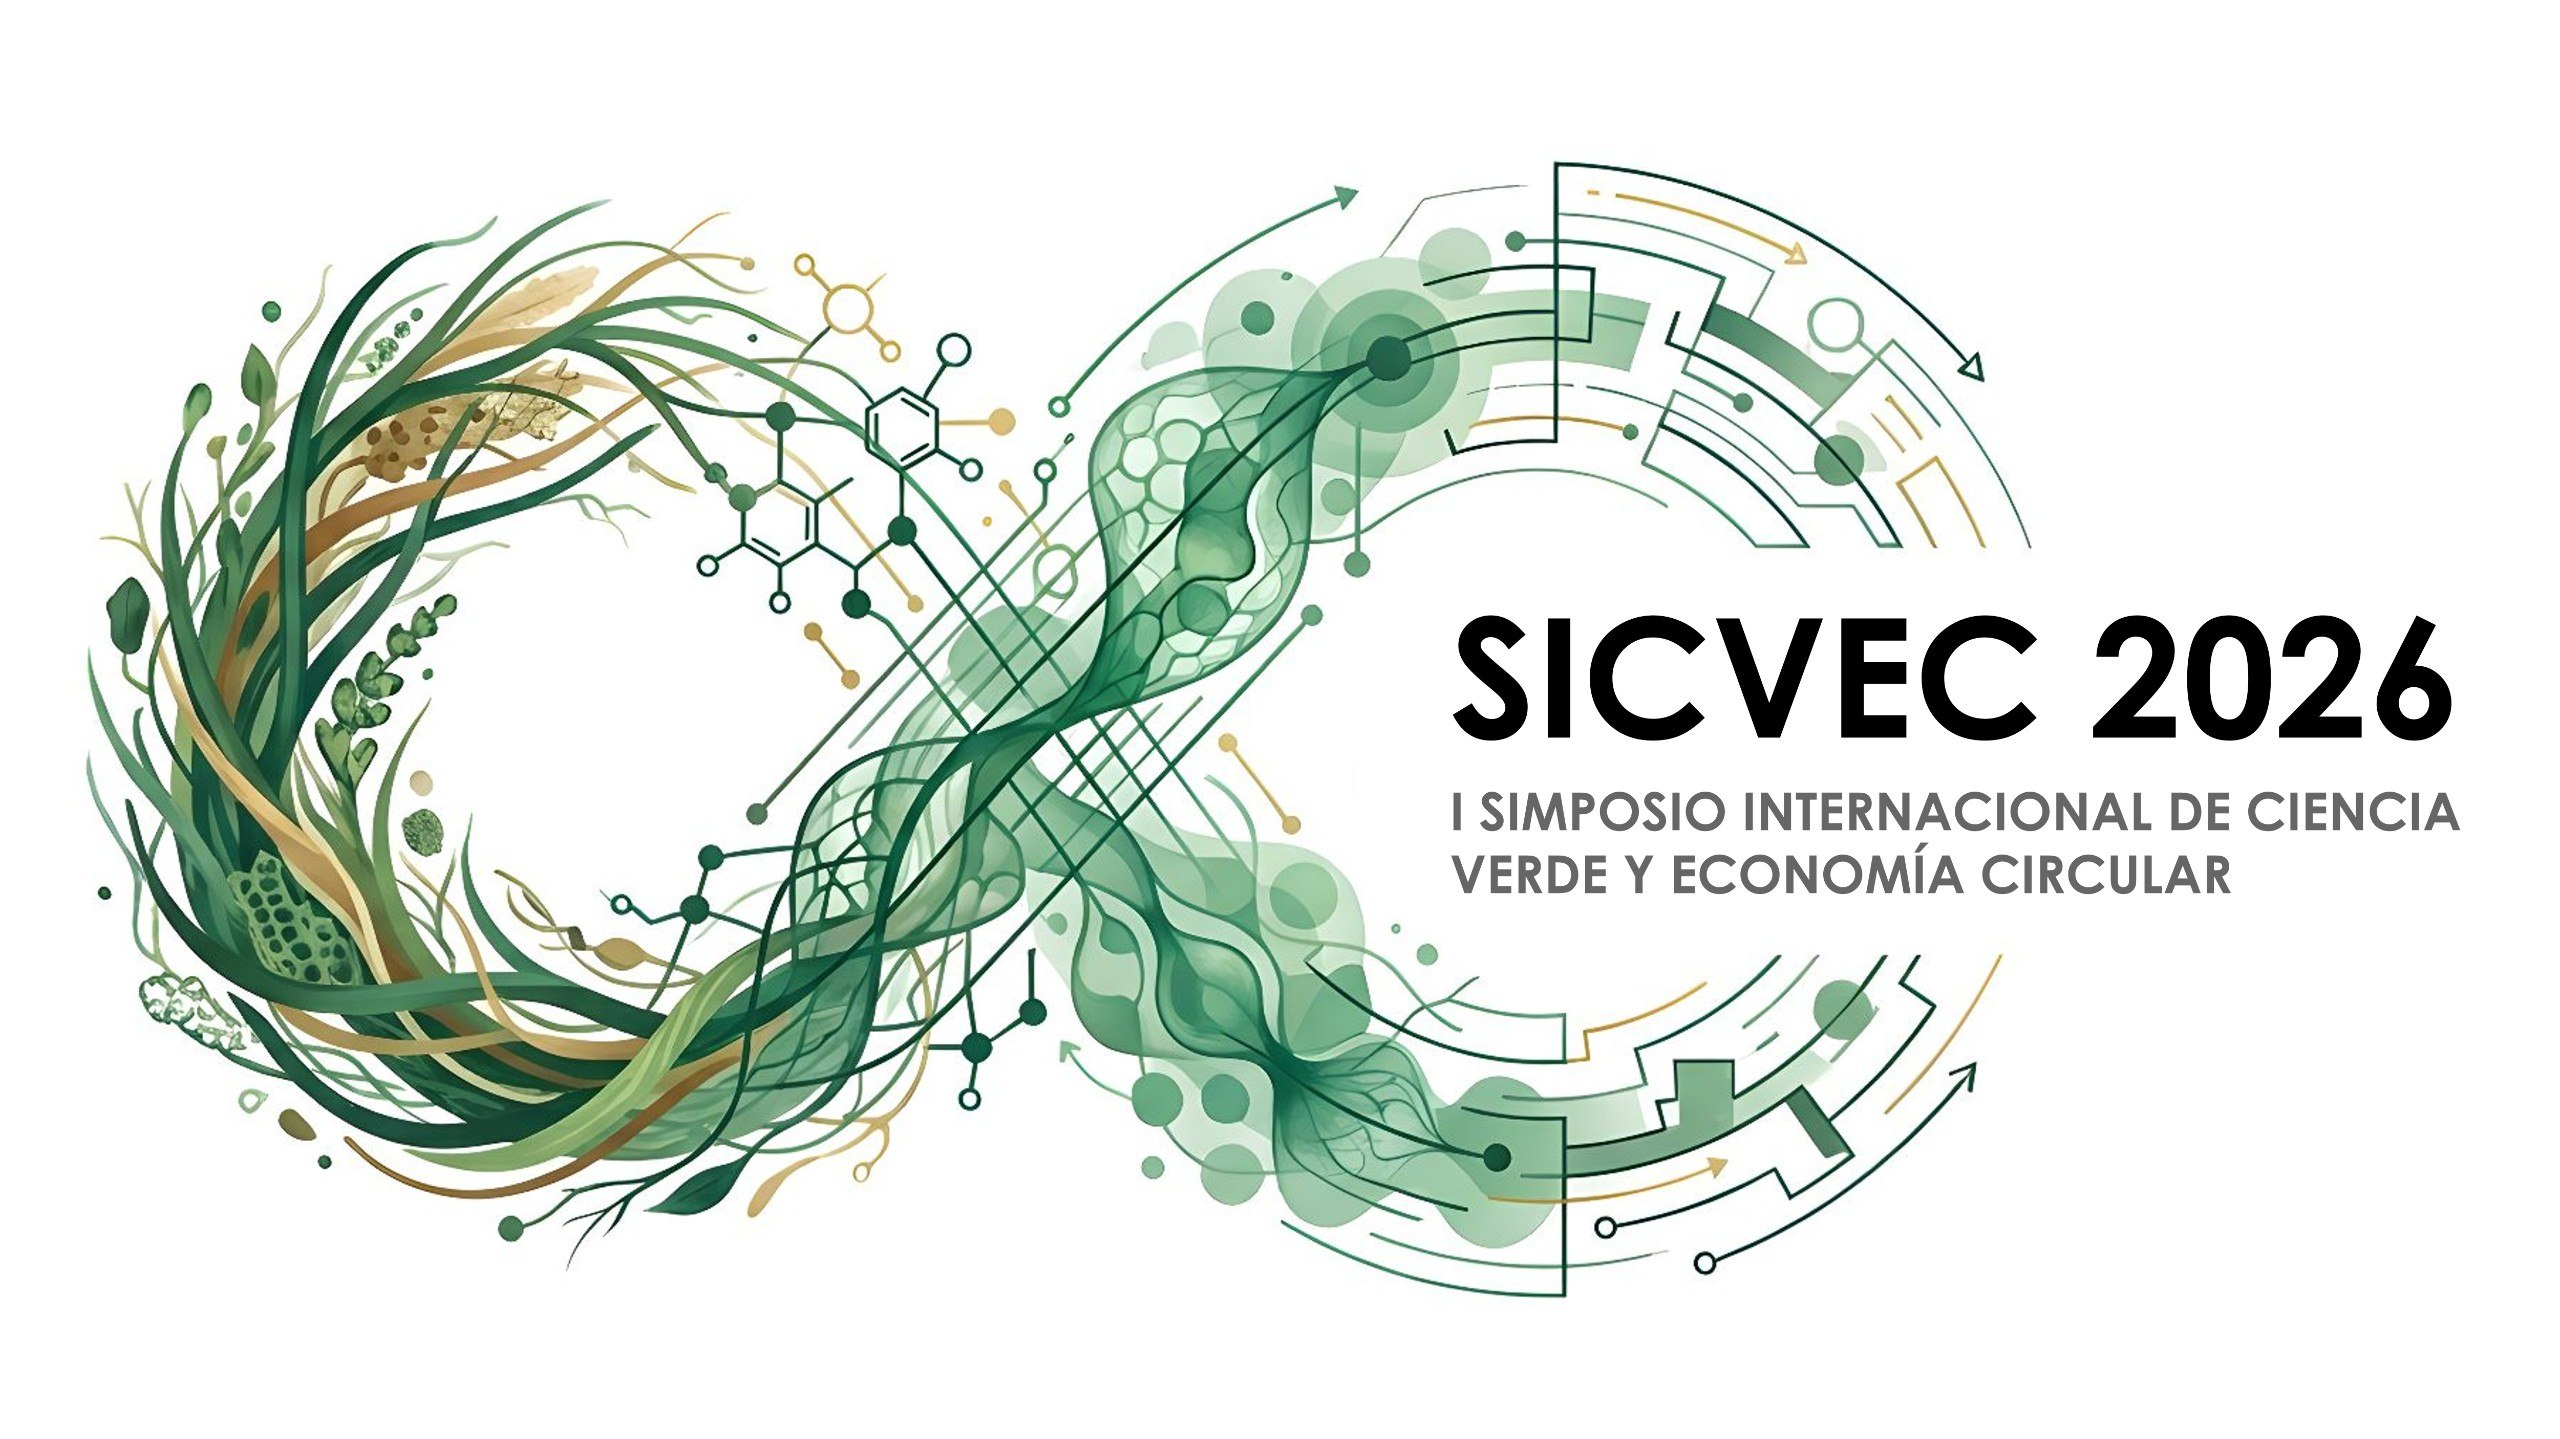
\includegraphics[height=0.8cm]{logo_sicvec2026.png} &
    
\includegraphics[height=0.8cm]{Logo_insilico.jpeg} \\
  \end{tabular*}%
}
\renewcommand{\headrulewidth}{1pt}
\renewcommand{\headrule}{\hbox to\headwidth{\color{verdeosc}\leaders\hrule height\headrulewidth\hfill}}

\begin{document}

\vspace{0.3cm}

\begin{center}
\textbf{\Large INTERNATIONAL SYMPOSIUM ON GREEN SCIENCE AND CIRCULAR ECONOMY}

\textbf{\large SICVEC 2026}

\textit{Brief for international partners and invited speakers}
\end{center}

\vspace{0.3cm}

\noindent
\textbf{THE EVENT}

\begin{tabular}{ll}
\textbf{Name:} & Simposio Internacional de Ciencia Verde y Economía Circular 2026 (SICVEC 2026) \\
\textbf{Dates:} & 19--20 October 2026 (Monday and Tuesday) \\
\textbf{Venue:} & Conference room, Centro Comercial Guacarí, Sincelejo, Sucre, Colombia \\
\textbf{Format:} & Hybrid: in person in Sincelejo + live online participation \\
\textbf{Attendance:} & 120--150 in-person participants + 300 online seats \\
\textbf{Organizer:} & Universidad de Sucre (UNISUCRE), Biology Programme, Faculty of Education and Sciences, \\
 & IN SILICO Research Group \\
\textbf{Languages:} & Spanish and English \\
\end{tabular}

\vspace{0.3cm}

\noindent
\textbf{AIM}

A meeting space for researchers, students and professionals in chemistry, physics, biology, mathematics,
environmental sciences and engineering to share research on sustainable processes, green chemistry,
biotechnology and circular economy, and to build inter-institutional collaborations. The symposium is
aligned with SDGs 12, 13, 15 and 17.

\vspace{0.3cm}

\noindent
\textbf{THEMATIC AXES}

\begin{enumerate}\setlength{\itemsep}{0.1cm}
\item Circular Economy: transition from linear to circular models, waste valorization, cascade economy, industrial symbiosis, life-cycle analysis.
\item Green Chemistry and Sustainable Processes: green synthesis, sustainable solvents, biocatalysis, clean processes, biomass valorization.
\item Sustainable Biotechnology: bioproducts, fermentation, green enzymes, biorefineries, bioplastics.
\item Green Technologies and Renewable Energy: clean energy, water treatment, environmental remediation, CO$_2$ capture.
\item Sustainability in Supply Chains: green certification, carbon footprint, cleaner production, agro-industrial innovation, short chains.
\item Public Policy and Environmental Governance: SDG 2030, regulatory frameworks, green incentives, environmental education.
\end{enumerate}

\vspace{0.2cm}

\noindent
\textbf{INVITED TALKS (KEYNOTES)}

Online, 45 minutes of presentation + 15 minutes of questions. Two keynotes per day (morning and afternoon).
Invited speakers are asked for: talk title and short abstract, a short biography and a profile photo
(for the programme and promotion), and confirmation of technical details before 1 October 2026.

\vspace{0.2cm}

\noindent
\textbf{CONTRIBUTED WORK (OPEN CALL)}

Oral presentations (20 minutes: 15 + 5 for questions) and posters, in Spanish or English, on any of the six axes.
Abstracts are peer reviewed and accepted work is published in the symposium proceedings.
Online participation is free of charge for external and international participants.

\vspace{0.2cm}

\noindent
\textbf{KEY DATES}

\begin{tabular}{ll}
Call for abstracts & 22 September -- 4 October 2026 (23:59, Colombia time) \\
Notification of acceptance & 8--9 October 2026 \\
Final material & 14 October 2026 \\
\textbf{Symposium} & \textbf{19--20 October 2026, 08:00--18:00 (UTC$-$5)} \\
Proceedings & 20 October 2026 \\
\end{tabular}

\vspace{0.2cm}

\noindent
\textbf{CONTACT}

\textbf{General Coordinator:} Dr. Aldo F. Combariza, IN SILICO Research Group, Universidad de Sucre.
Email: \href{mailto:aldo.combariza@unisucre.edu.co}{aldo.combariza@unisucre.edu.co}
(coordination: \href{mailto:insilico@unisucre.edu.co}{insilico@unisucre.edu.co}).

Event website and abstract submission platform: to be announced.

\end{document}
